\documentclass{beamer}
\usepackage{hyperref}
\usepackage[T1]{fontenc}
\usepackage{latexsym,amsmath,xcolor,multicol,booktabs,calligra}
\usepackage{graphicx,pstricks,listings,stackengine}
\usepackage{tikz}

\author{Kirill Zemlianskii}
\title{Assessing Synthetic Benchmark Reliability}
\subtitle{A Case Study on the Canon Layer}
\institute{}
\date{June 2026}
\usepackage{CNU}
% CNU theme references CJK font families (defined via ctex in the author's
% environment); provide ASCII fallbacks so the deck builds standalone.
\def\kaishu{\rmfamily}
\def\heiti{\sffamily\bfseries}
\setbeamertemplate{headline}{}

% Suppress auto-generated ToC frames at each section
\AtBeginSection{}

\definecolor{deepblue}{rgb}{0,0,0.5}
\definecolor{deepred}{rgb}{0.6,0,0}
\definecolor{deepgreen}{rgb}{0,0.5,0}
\definecolor{halfgray}{gray}{0.55}
\definecolor{CNUblue}{HTML}{3434b4}

% Figures: new paper plots live in ./plots/, static art under ../plots/
\graphicspath{{plots/}{../plots/}}

\begin{document}

% ------------------------------------------------------------------
% Slide 1 --- Title
% ------------------------------------------------------------------
\begin{frame}
  \titlepage
\end{frame}


% ==================================================================
\section{Motivation}
% ==================================================================

% ------------------------------------------------------------------
% Slide 2 --- The Architecture Zoo Problem
% ------------------------------------------------------------------
\begin{frame}{The Architecture Zoo Problem}
  \textbf{A wide range of architectural changes:}
  \begin{itemize}
    \item Attention: sliding-window, MLA (DeepSeek), gated attention, DSA
    \item Positional encoding: RoPE, NoPE, ALiBi
    \item Gating: gated MLP, SwiGLU, MoE
  \end{itemize}

  \vspace{0.6em}
  \textbf{The difficulty in comparing}
  \begin{itemize}
    \item Costly training
    \item Noisy benchmarks
    \item Overlapping results, with no clear winner overall
  \end{itemize}
\end{frame}


% ==================================================================
\section{Synthetic Data as a Solution}
% ==================================================================

% ------------------------------------------------------------------
% Slide 3 --- The Synthetic Playground Idea
% ------------------------------------------------------------------
\begin{frame}{The Synthetic Playground}
  \begin{columns}[T]
    \column{0.55\textwidth}
      \textbf{Idea:} Decompose ``reasoning'' into atomic skills;
      design one controlled task per skill.

      \vspace{0.5em}
      \textbf{Advantages:}
      \begin{itemize}
        \item Generation on-the-fly, no need for storage
        \item Can be trained to achieve reasonable accuracy on small scale.
        \item Controlled difficulty
      \end{itemize}

      \vspace{0.4em}
      \small Motivation: A task mirrors real capability of a model needed for text modeling

    \column{0.42\textwidth}
      \textbf{Tasks used in this study}
      \vspace{0.3em}
      \begin{center}
      \begin{tabular}{@{}ll@{}}
        \toprule
        \textbf{Depo} & Reasoning depth \\
        ConComp & Reasoning depth \\
        ShortPath & Reasoning breadth \\
        BFS & Reasoning breadth \\
        \bottomrule
      \end{tabular}
      \end{center}
      \small Each graph task in two encodings (edges-list / adj-list) $\Rightarrow$ 8 variants.
  \end{columns}
\end{frame}


% ==================================================================
\section{Task Descriptions}
% ==================================================================

% ------------------------------------------------------------------
% Slide 4 --- Task Depo
% ------------------------------------------------------------------
\begin{frame}{Task Depo: Multi-hop Retrieval}
  \begin{columns}[T]
    \column{0.38\textwidth}
      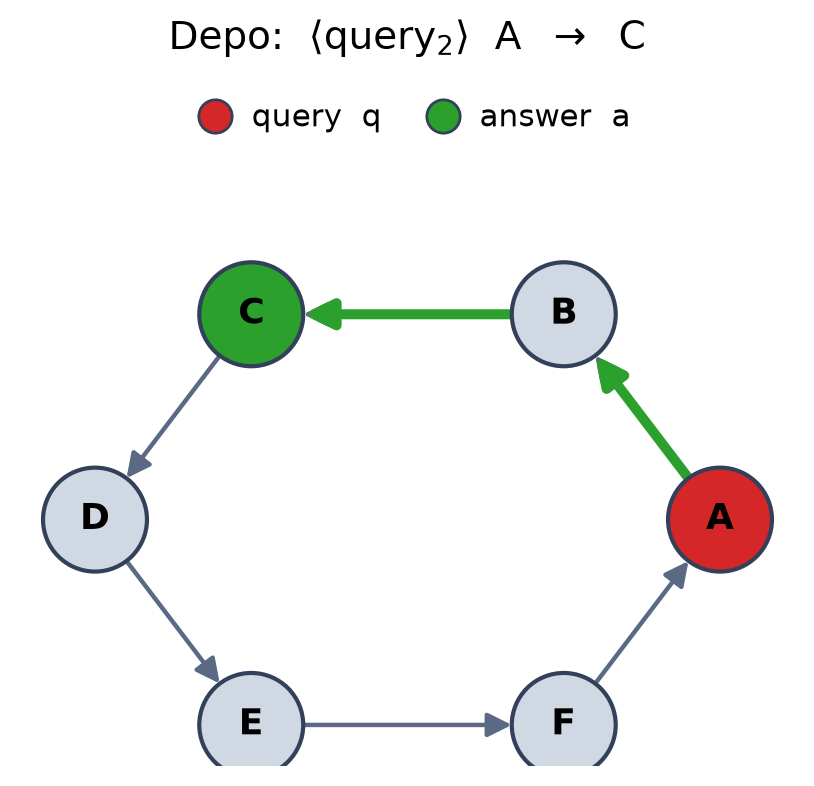
\includegraphics[width=\linewidth]{task_example_depo.png}
    \column{0.6\textwidth}
      \textbf{Setup:} $k$-hop traversal over a directed permutation graph.
      No Chain-of-Thought; node labels span multiple tokens.

      \vspace{0.4em}
      \textbf{Format (edges-list):}
      \[
        \texttt{<bos>}\ A\,B\ \ C\,D\ \cdots\
        \texttt{<query\_2>}\ \textcolor{deepred}{A} \to \textcolor{deepgreen}{C}
      \]
      \textbf{Format (adj-list):}
      \[
        \texttt{<bos>}\ A\,\texttt{<sep>}\,B\ \cdots\
        \texttt{<query\_2>}\ \textcolor{deepred}{A} \to \textcolor{deepgreen}{C}
      \]

      \vspace{0.4em}
      \begin{itemize}
        \item Chain $k$ retrievals in activations; no output tokens
        \item Must represent the whole graph
      \end{itemize}
  \end{columns}
\end{frame}

% ------------------------------------------------------------------
% Slide 4b --- Task ConComp
% ------------------------------------------------------------------
\begin{frame}{Task ConComp: Component Factorisation}
  \begin{columns}[T]
    \column{0.38\textwidth}
      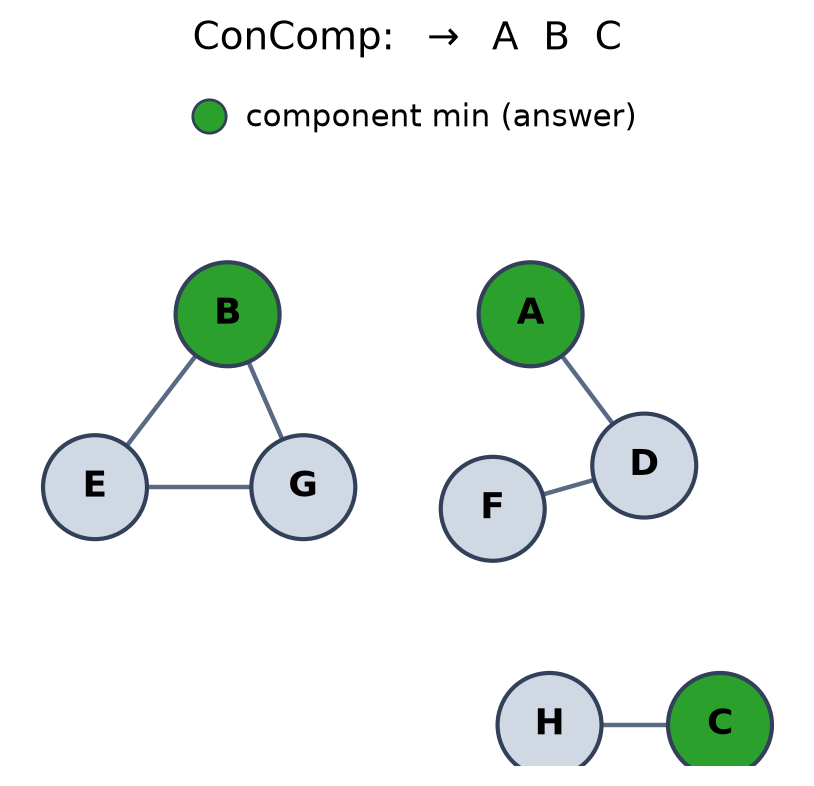
\includegraphics[width=\linewidth]{task_example_concomp.png}
    \column{0.6\textwidth}
      \textbf{Setup:} Undirected random graph (up to 50 nodes, multiple
      components). Multi-token node labels.

      \vspace{0.4em}
      \textbf{Format:}
      \[
        \texttt{<task>}\ G\ \texttt{<sep>}
        \;\to\;
        \textcolor{deepgreen}{A}\ \textcolor{deepgreen}{B}\
        \textcolor{deepgreen}{C}\ \texttt{<eos>}
      \]
      Output $r_i$: the lexicographically smallest node in component $i$, one
      per component in traversal order.

      \vspace{0.4em}
      \begin{itemize}
        \item Partition the graph globally into disjoint components
        \item Must build a representation of the whole graph
      \end{itemize}
  \end{columns}
\end{frame}

% ------------------------------------------------------------------
% Slide 4c --- Task ShortPath
% ------------------------------------------------------------------
\begin{frame}{Task ShortPath: Shortest-Path Planning}
  \begin{columns}[T]
    \column{0.38\textwidth}
      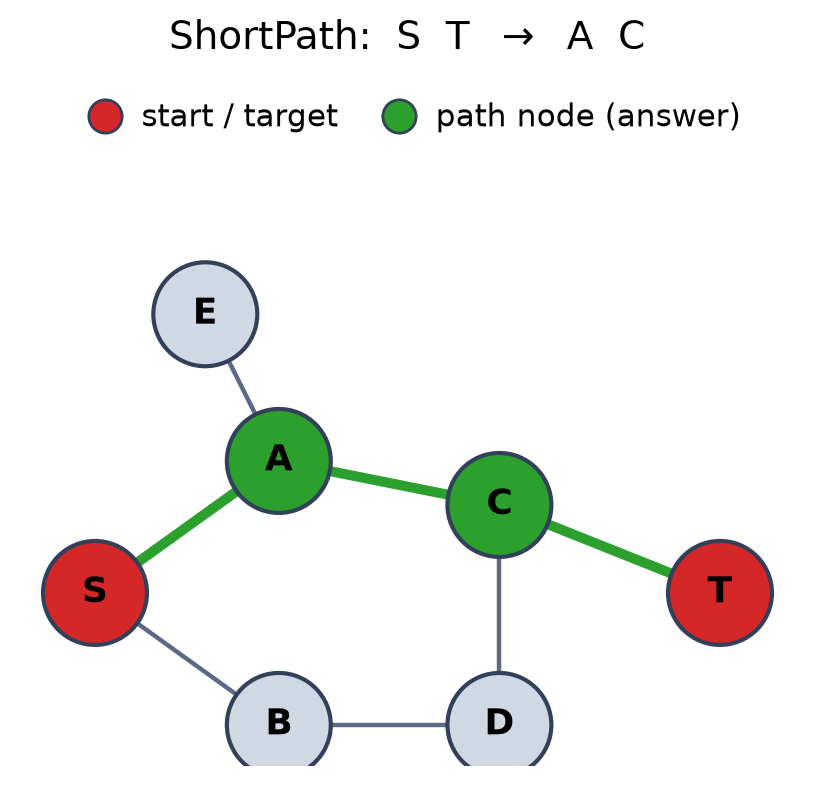
\includegraphics[width=\linewidth]{task_example_shortpath.png}
    \column{0.6\textwidth}
      \textbf{Setup:} Undirected random graph. Start node $s$ and target node
      $t$ at BFS distance $d$.

      \vspace{0.4em}
      \textbf{Format:}
      \[
        \texttt{<task>}\ G\ \texttt{<sep>}\
        \textcolor{deepred}{S}\ \textcolor{deepred}{T}
        \;\to\;
        \textcolor{deepgreen}{A}\ \textcolor{deepgreen}{C}\ \texttt{<eos>}
      \]
      Output the intermediate nodes on the shortest path from $s$ to $t$
      (start excluded).

      \vspace{0.4em}
      \begin{itemize}
        \item Step-by-step planning along valid graph edges
        \item Difficulty set by path length / target distance
      \end{itemize}
  \end{columns}
\end{frame}

% ------------------------------------------------------------------
% Slide 4d --- Task BFS
% ------------------------------------------------------------------
\begin{frame}{Task BFS: Breadth-First Traversal}
  \begin{columns}[T]
    \column{0.38\textwidth}
      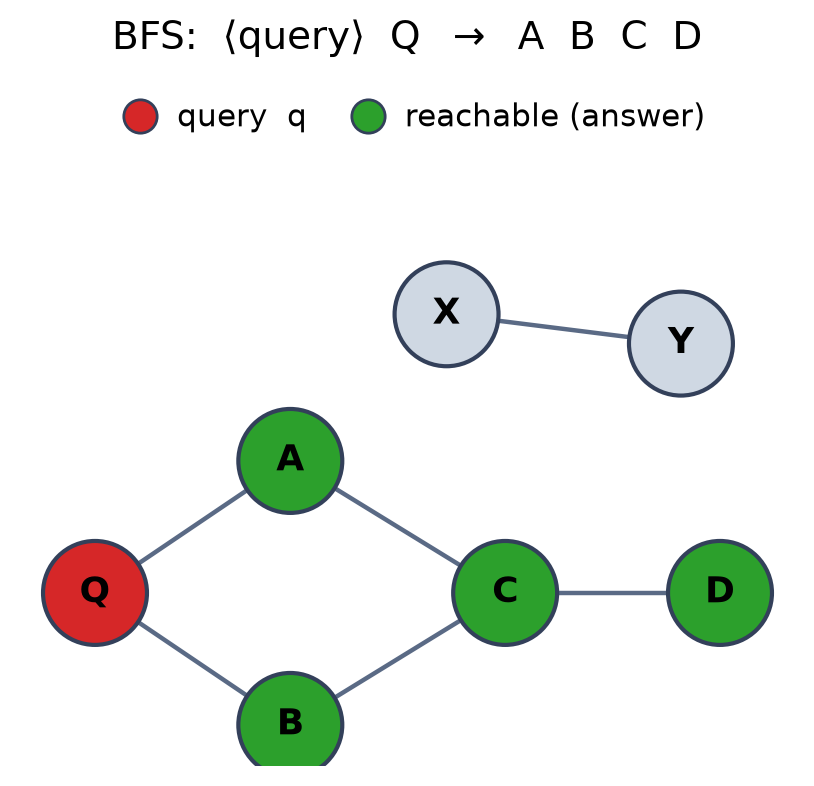
\includegraphics[width=\linewidth]{task_example_bfs.png}
    \column{0.6\textwidth}
      \textbf{Setup:} Undirected random graph. A single query node $q$.

      \vspace{0.4em}
      \textbf{Format:}
      \[
        \texttt{<task>}\ G\ \texttt{<query>}\ \textcolor{deepred}{Q}
        \;\to\;
        \textcolor{deepgreen}{A}\ \textcolor{deepgreen}{B}\
        \textcolor{deepgreen}{C}\ \textcolor{deepgreen}{D}\ \texttt{<eos>}
      \]
      Enumerate all nodes reachable from $q$ in BFS discovery order
      (capped at $n_{\max}$).

      \vspace{0.4em}
      \begin{itemize}
        \item Step-by-step planning along valid graph edges
        \item Difficulty set by the number of reachable nodes
      \end{itemize}
  \end{columns}
\end{frame}

% ------------------------------------------------------------------
% Slide 5 --- Graph-search tasks
% ------------------------------------------------------------------
\begin{frame}{Graph-search Tasks \& Encodings}
  \textbf{Sequential tasks} (each over a random graph, answer tokens only):
  \begin{itemize}
    \item \textbf{ShortestPath:} output a shortest path between two nodes
    \item \textbf{BFS:} output the set of nodes reachable from a query node
    \item \textbf{ConComp:} output one node per connected component
  \end{itemize}
  \textbf{Single answer node tasks} (Model produces a single answer node):
  \begin{itemize}
    \item \textbf{Depo:} output the k-th successor node of a query node
  \end{itemize}

  \vspace{0.5em}
  \textbf{Two encodings of the same graph:}
  \begin{itemize}
    \item \texttt{edges\_list}: a flat list of edges
    \item \texttt{adj\_list}: per-node adjacency
  \end{itemize}

\end{frame}


% ==================================================================
\section{Canon Layers}
% ==================================================================

% ------------------------------------------------------------------
% Slide 6 --- Canon Layer Design
% ------------------------------------------------------------------
\begin{frame}{Canon Layers: Design}
  \textbf{Motivation:} Insufficient horizontal mixing in the transformer.

  \vspace{0.4em}
  \textbf{Solution:} a lightweight depthwise causal convolution on the
  residual stream:
  \[
    \tilde h_t = \sum_{j=0}^{k-1} w_j \odot h_{t-j}
    \qquad (k \text{ taps, weights shared across channels})
  \]

  \vspace{0.4em}
  \textbf{Implementation:}
  \begin{itemize}
    \item Causal convolution, kernel size $k$ (default 4) + residual standard torch Conv1d init
    \item Negligible parameter overhead
    \item Enables horizontal mixing
  \end{itemize}
\end{frame}

% ------------------------------------------------------------------
% Slide 6b --- Canon Layer Insertion Points
% ------------------------------------------------------------------
\begin{frame}{Canon Layers: Insertion Points}
  \begin{columns}[T]
    \column{0.48\textwidth}
      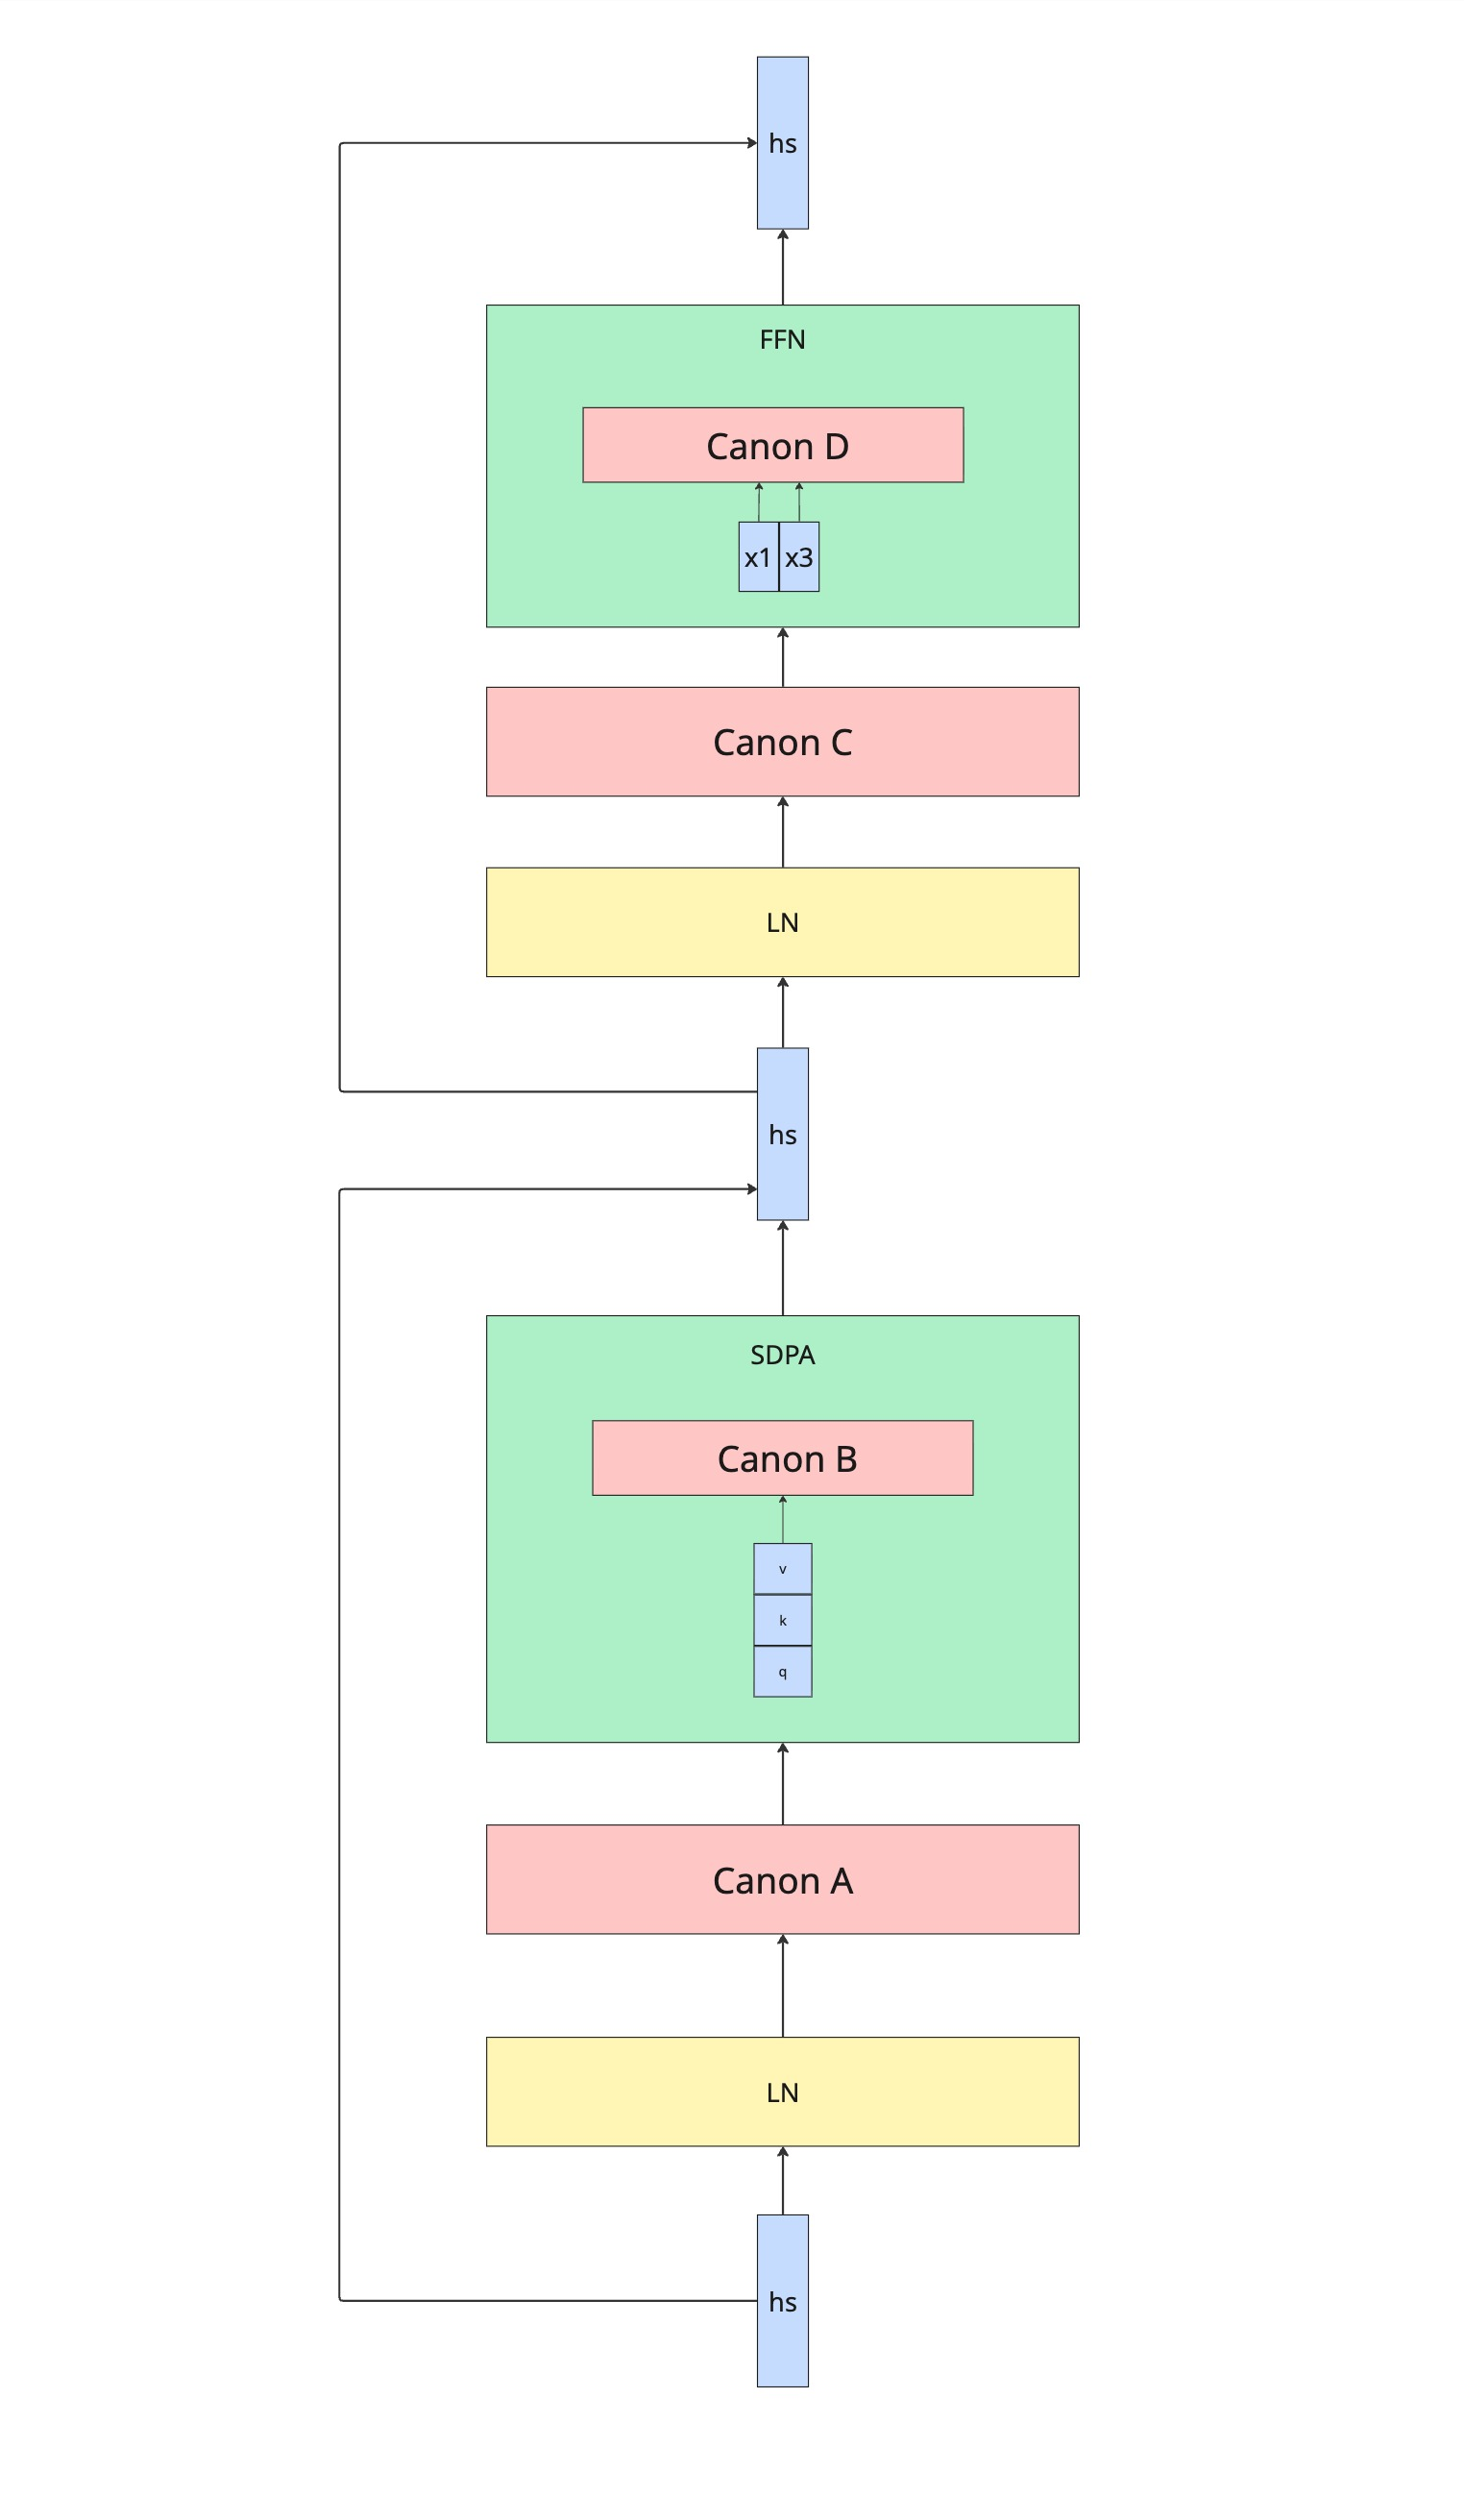
\includegraphics[width=\linewidth]{canon_location_scheme.jpg}

    \column{0.48\textwidth}
      \textbf{4 insertion points per transformer block:}
      \begin{itemize}
        \item[\textbf{A}] Pre-attention
        \item[\textbf{B}] Post-attention
        \item[\textbf{C}] Pre-FFN
        \item[\textbf{D}] Post-FFN
      \end{itemize}
      \vspace{0.4em}
      The full configuration \textbf{Canon-ABCD} places one at every position,
      and this is the configuration we study throughout.
  \end{columns}
\end{frame}

% ------------------------------------------------------------------
% Slide 7 --- Motivation: re-examine the claims
% ------------------------------------------------------------------
\begin{frame}{Canon: Motivation to Re-examine}
  The original Physics 4.1 work (Allen-Zhu \& Li) presents Canon as a broadly useful
  primitive, validated \emph{on exactly these synthetic benchmarks}, but leaves
  open \emph{why} it works.

  \vspace{0.8em}
  \textbf{We use Canon as a running example to ask two things:}
  \begin{itemize}
    \item Can the benchmarks be used to compare canon with baseline llama? Are results aligned with text modeling?
    \item When does canon improve perforamnce? Can we use benchmarks to study training dynamics and interpret the layer?
  \end{itemize}
\end{frame}


% ==================================================================
\section{Setup}
% ==================================================================

% ------------------------------------------------------------------
% Slide 8 --- Setup
% ------------------------------------------------------------------
\begin{frame}{Experimental Setup}
  \begin{columns}[T]
    \column{0.5\textwidth}
      \textbf{Framework:} Meta Lingua (\texttt{lingua\_modified})

      \textbf{Canon Implementation:} CUDA kernel from Dao-AILab/causal-conv1d

      \vspace{0.4em}
      \textbf{Models:} LLama model. RoPE position encoding, tied embeddings, MHA, Pre-LN, SwiGLU activations

      \vspace{0.4em}
      \textbf{Scales:} 3M, 10M, 30M, 100M parameters \\


    \column{0.47\textwidth}
      \textbf{Benchmark:} 8-task mix\\(4 graph tasks $\times$ 2 encodings)
      \textbf{Optimization:} AdamW, 3e-4 LR, 100k steps, cosine scheduling, beta1=0.9, beta2=0.98, epsilon=1e-6.
      \end{columns}

\end{frame}


% ==================================================================
\section{Part 1: Can the Measurement Be Trusted?}
% ==================================================================

% ------------------------------------------------------------------
% Slide 9 --- A single run is unreliable: grokking
% ------------------------------------------------------------------
\begin{frame}{Seed variability}
  \begin{columns}[T]
    \column{0.5\textwidth}
      
\includegraphics[width=\linewidth]{text_stable.png}
      \begin{center}\small Text: seeds nearly identical\end{center}
    \column{0.5\textwidth}
      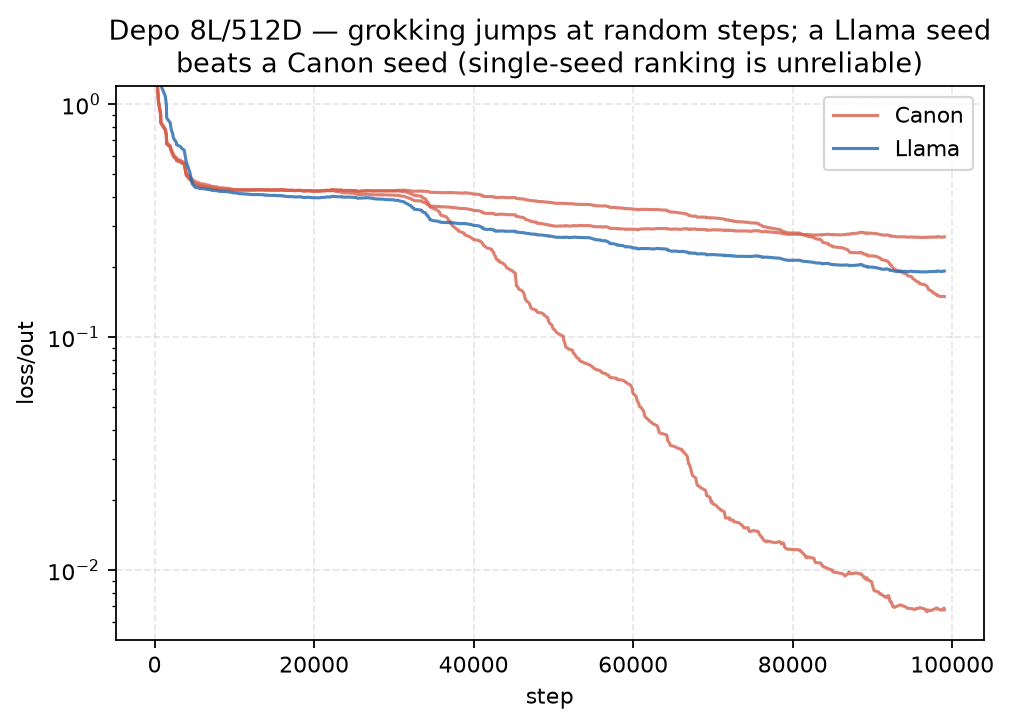
\includegraphics[width=\linewidth]{depo_grokking.png}
      \begin{center}\small Depo: grokking at random steps\end{center}
  \end{columns}
  \vspace{0.2em}
  \begin{itemize}
    \item Text modelling is a stable reference: Canon is reliably better than Llama
    \item On Depo the grokking occurs at random steps
    \item Some runs of Canon are worse than baseline Llama
  \end{itemize}
\end{frame}

% ------------------------------------------------------------------
% Slide 10 --- Variance localised to Depo
% ------------------------------------------------------------------
\begin{frame}{Instability is Linked to Grokking}
  \begin{center}
    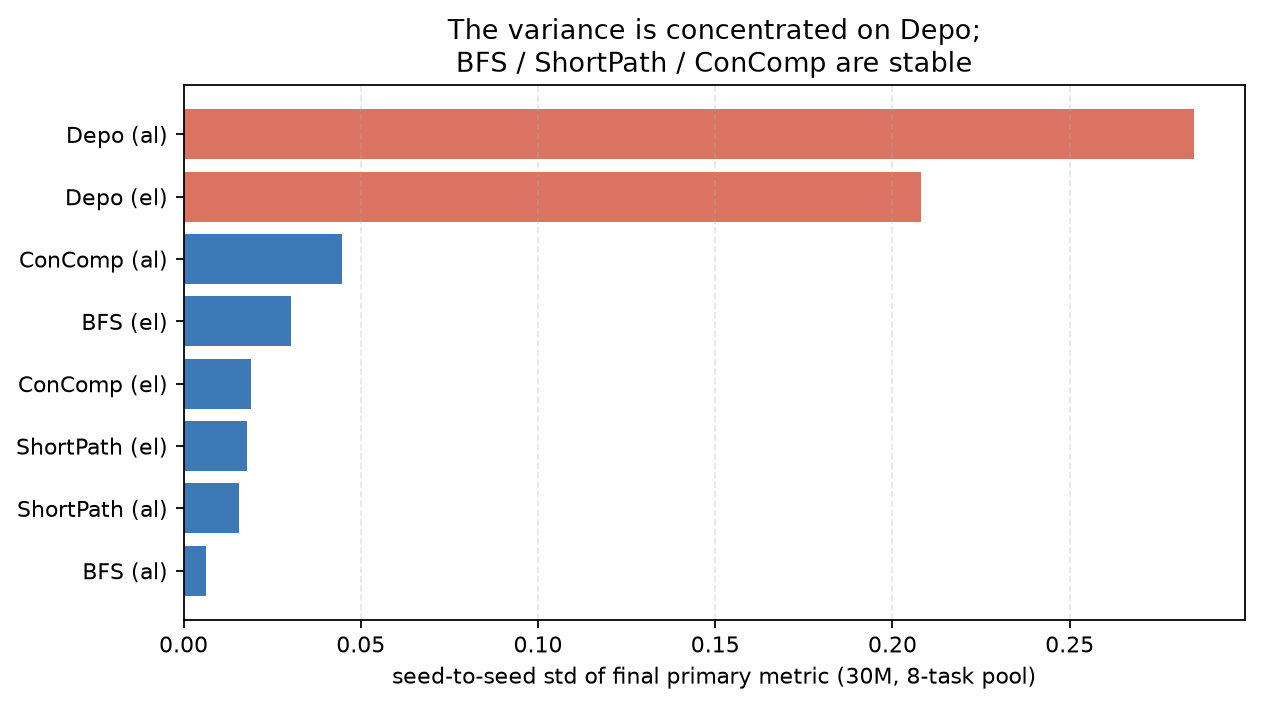
\includegraphics[width=0.6\linewidth]{task_noise.png}\\
    \small Final-score spread, by task
  \end{center}
  \vspace{0.2em}
  \begin{itemize}
    \item Instability is associated with grokking: tasks that don't grok stay much more stable.
  \end{itemize}
\end{frame}


% ==================================================================
\section{Part 1: The Verdict, Done Right}
% ==================================================================

% ------------------------------------------------------------------
% Slide 11 --- Scaling
% ------------------------------------------------------------------
\begin{frame}{High variance requires more runs; Canon beats Llama}
  \begin{columns}[T]
    \column{0.55\textwidth}
      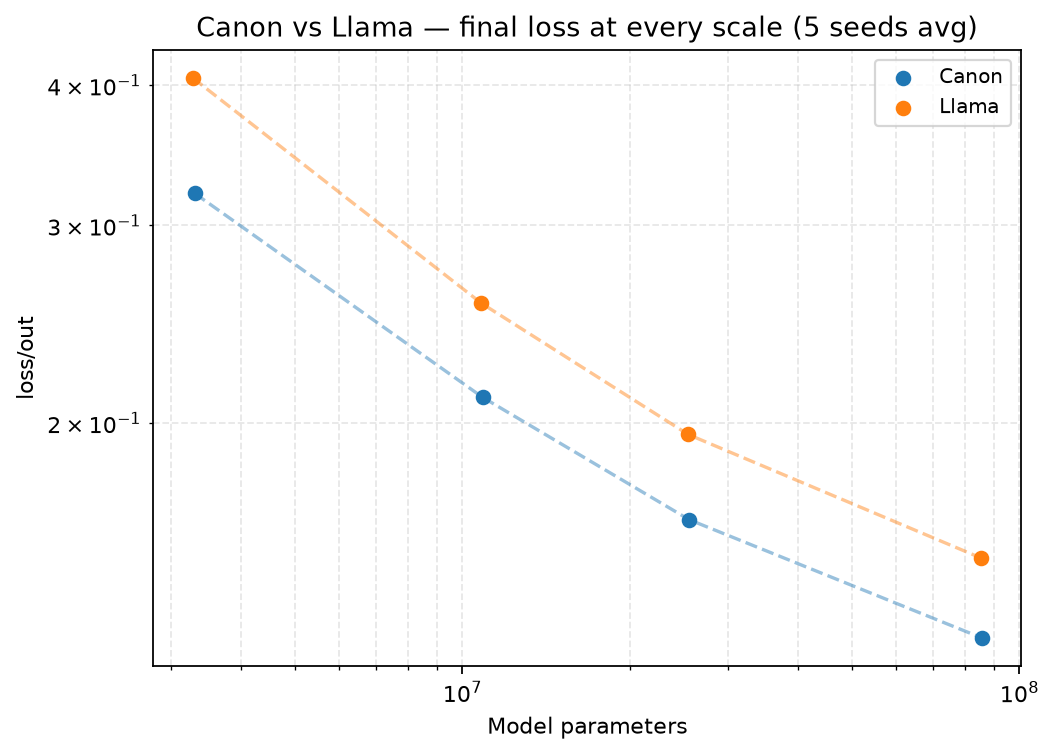
\includegraphics[width=\linewidth]{scaling.png}
    \column{0.43\textwidth}
      \textbf{Canon scaling} (5 seeds averaged per point).
      \begin{itemize}
        \item Canon beats Llama at every scale: 3M, 10M, 30M, 100M.
        \item Required 5 runs per model / size for fair comparison.
      \end{itemize}
  \end{columns}
\end{frame}

% ------------------------------------------------------------------
% Slide 12 --- Where Canon helps
% ------------------------------------------------------------------
\begin{frame}{Most significant gain on depth of reasoning tasks}
  \begin{center}
    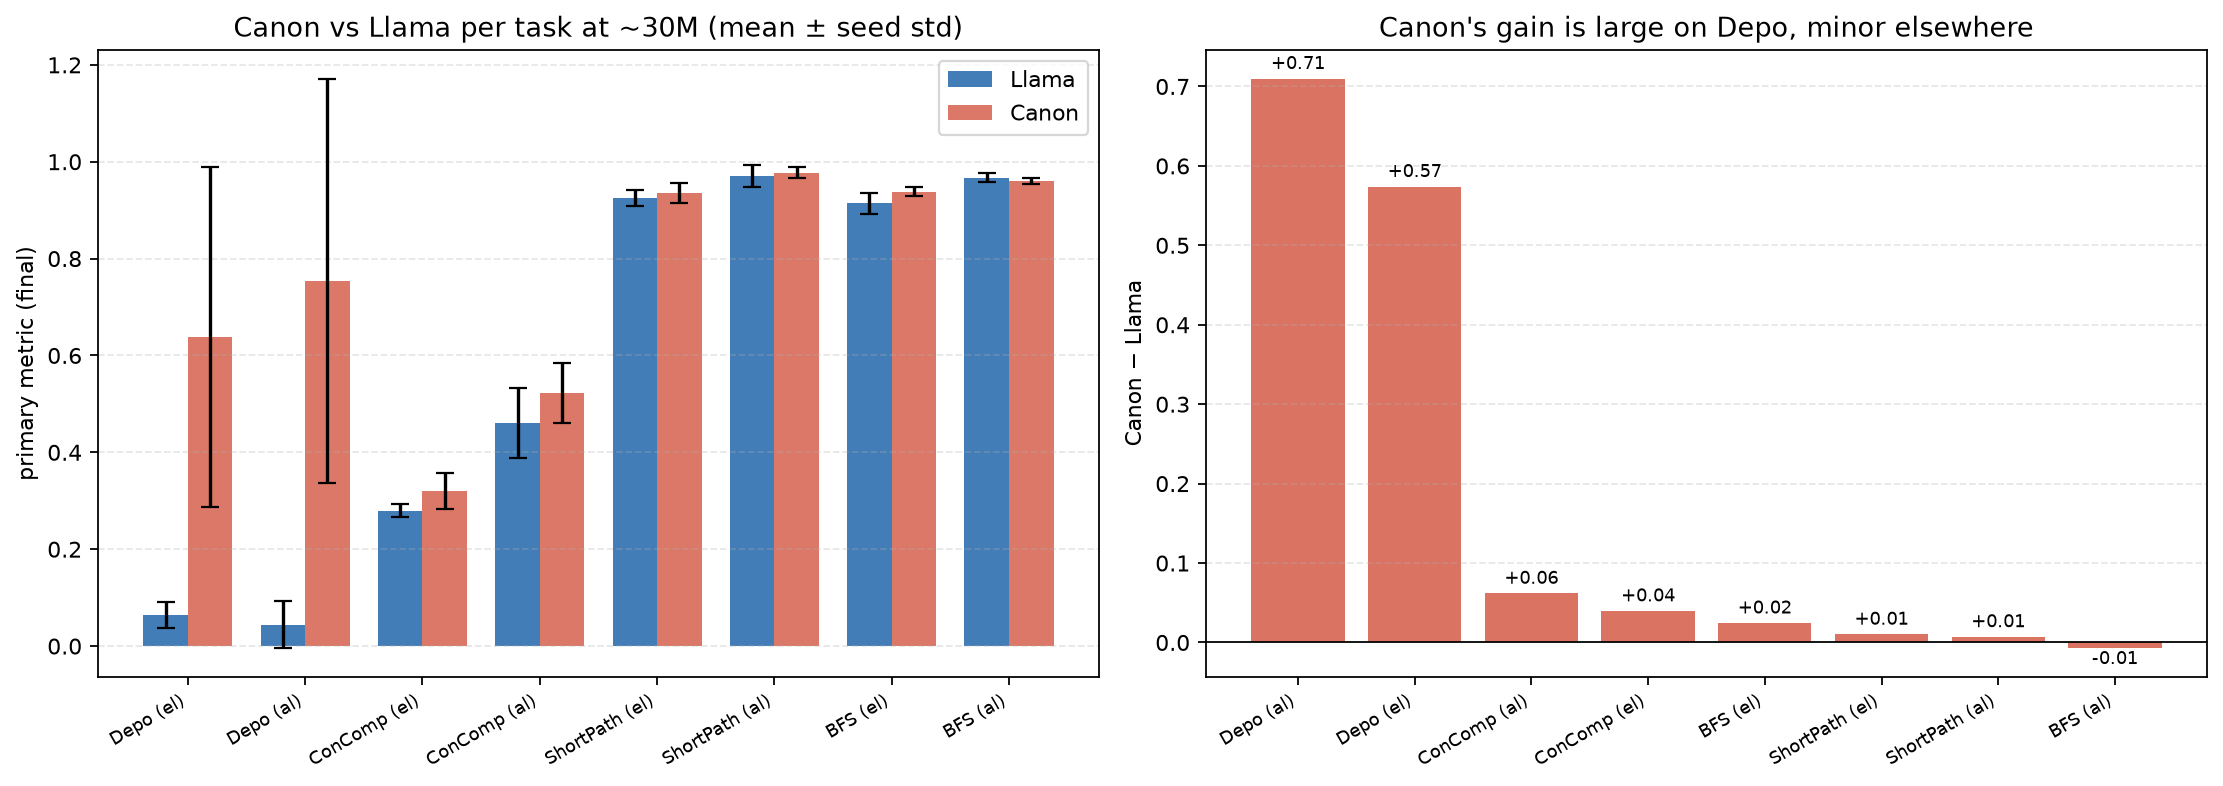
\includegraphics[width=0.92\linewidth]{task_breakdown.png}
  \end{center}
  \vspace{0.1em}
  \begin{itemize}
    \item Depo and ConComp require building representation of the whole graph in one step.
    \item Those tasks show the largest gain with Canon, while ConComp is much more stable than Depo.
    \item Depo has the highest correlation with ConComp
  \end{itemize}
\end{frame}


% ==================================================================
\section{Part 2: Mechanism --- Studied on Text}
% ==================================================================

% ------------------------------------------------------------------
% Slide 13a --- Hope: dynamics are less seed-volatile, qualitatively agree
% ------------------------------------------------------------------
\begin{frame}{Training dynamics interpretation}
  \begin{columns}[T]
    \column{0.34\textwidth}
      \small
      Maybe we can use the benchmarks to interpret architectural changes.

      \vspace{0.5em}
      \textbf{Some encouragement:} Some of the qualitative dynamics changes persist between runs and are consistent between text and synthetic.

    \column{0.64\textwidth}
      \centering
      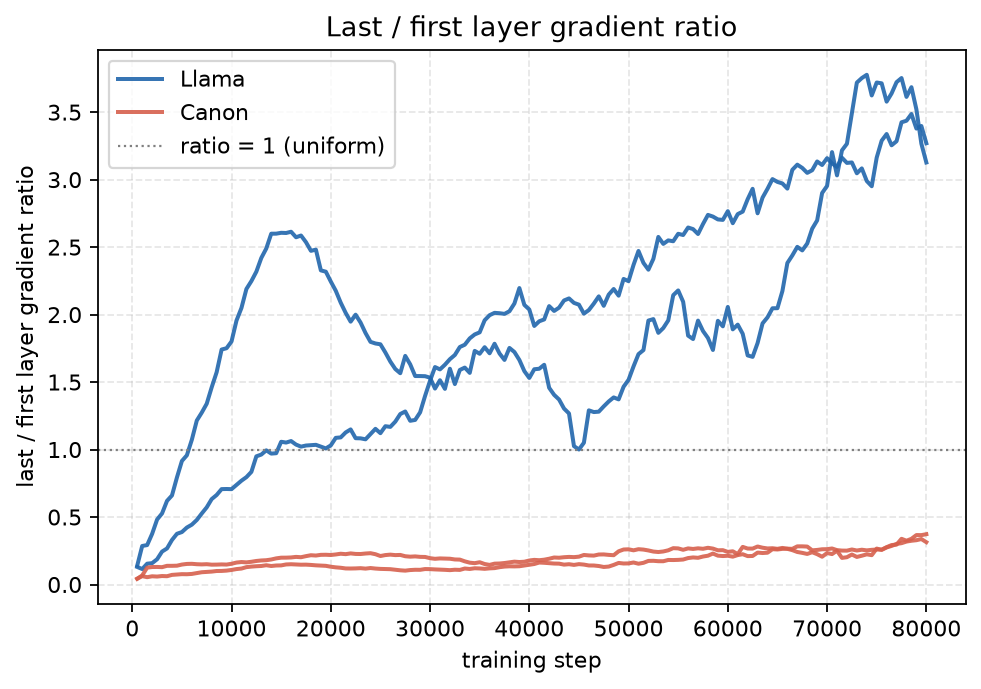
\includegraphics[height=0.34\textheight]{grad_ratio_seeds.png}\\[-0.2em]
      {\small Last/first layer gradient ratio (synthetic, different seeds)}

      \vspace{0.3em}
      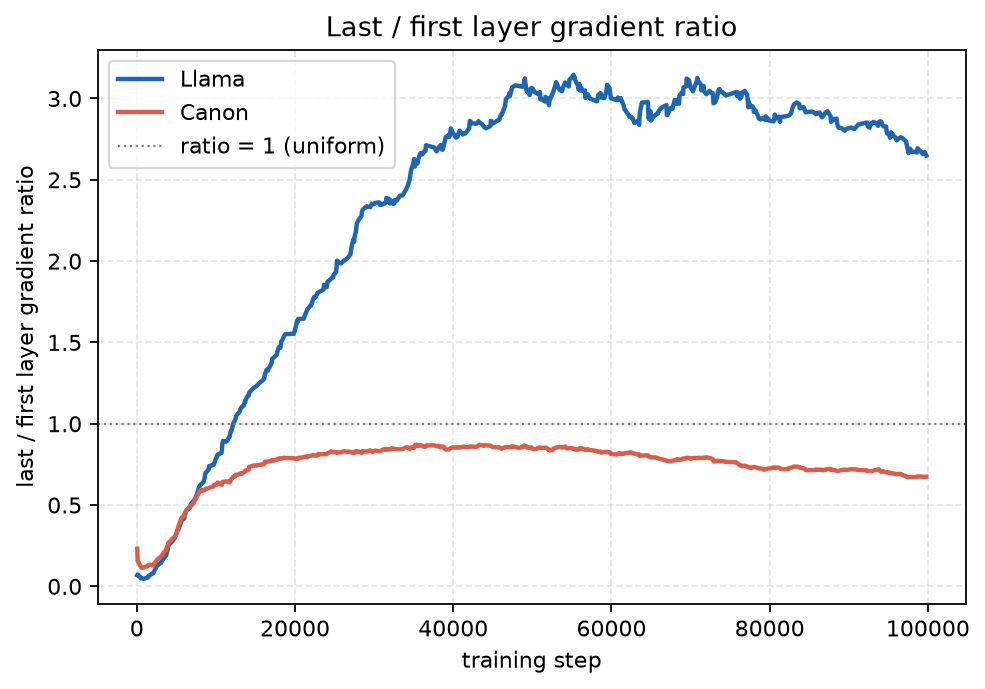
\includegraphics[height=0.34\textheight]{grad_ratio.png}\\[-0.2em]
      {\small Last/first layer gradient ratio (text)}
  \end{columns}
\end{frame}

% ------------------------------------------------------------------
% Slide 13b --- But the key mechanisms do NOT reproduce synthetically
% ------------------------------------------------------------------
\begin{frame}{Training dynamics interpretation}
  \begin{columns}[T]
    \column{0.5\textwidth}
      \begin{center}\small \textbf{Gradient profile}\end{center}
      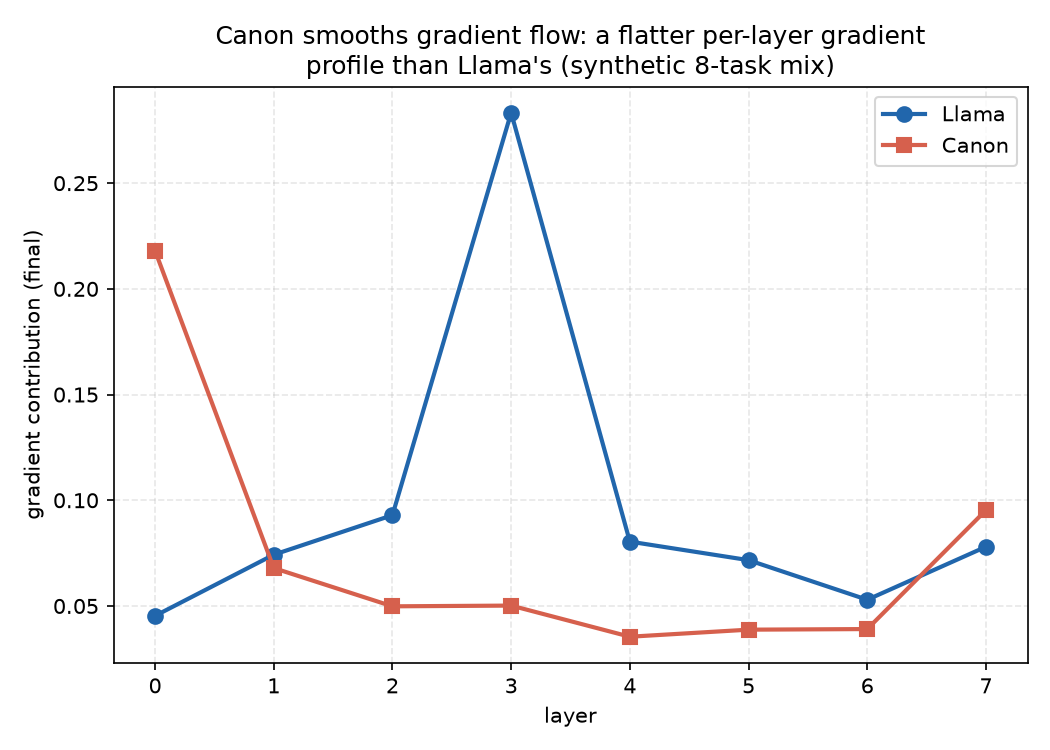
\includegraphics[width=0.49\linewidth]{grad_profile_synth.png}\hfill
      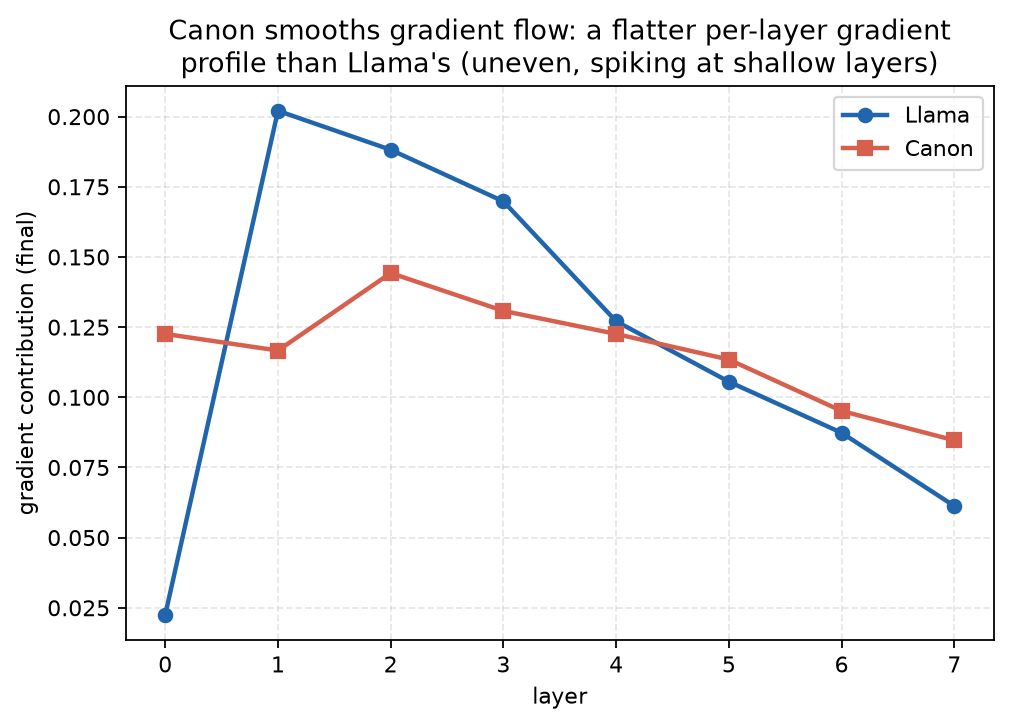
\includegraphics[width=0.49\linewidth]{grad_profile.png}\\[-0.1em]
      {\centering\scriptsize\hspace*{0.18\linewidth}synthetic\hfill text\hspace*{0.14\linewidth}\par}
    \column{0.5\textwidth}
      \begin{center}\small \textbf{Representation (RMS) ratio}\end{center}
      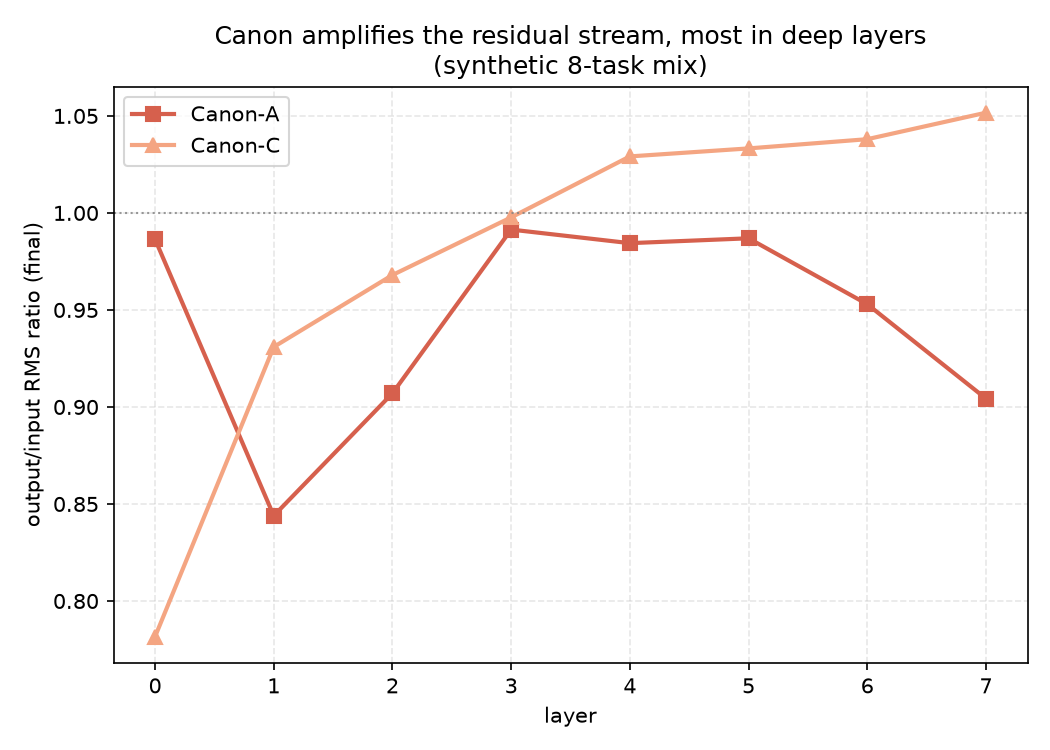
\includegraphics[width=0.49\linewidth]{rms_ratio_synth.png}\hfill
      
\includegraphics[width=0.49\linewidth]{rms_ratio.png}\\[-0.1em]
      {\centering\scriptsize\hspace*{0.18\linewidth}synthetic\hfill text\hspace*{0.14\linewidth}\par}
  \end{columns}
  \vspace{0.2em}
  \begin{itemize}\small
    \item However, the most interesting mechanistic results we saw on text do not
          reproduce synthetically
    \item Conclusions are hard to draw. Training dynamics on sythetic tasks differ from text.
    \item[$\Rightarrow$] Further we focus on studying canon on text to gain more reliable insights.
  \end{itemize}
\end{frame}

% ------------------------------------------------------------------
% Slide 14 --- Mechanisms 1 & 2: gradient smoothing + representation upscaling
% ------------------------------------------------------------------
\begin{frame}{Mechanisms: Gradient Smoothing \& Representation Upscaling}
  \begin{columns}[T]
    \column{0.5\textwidth}
      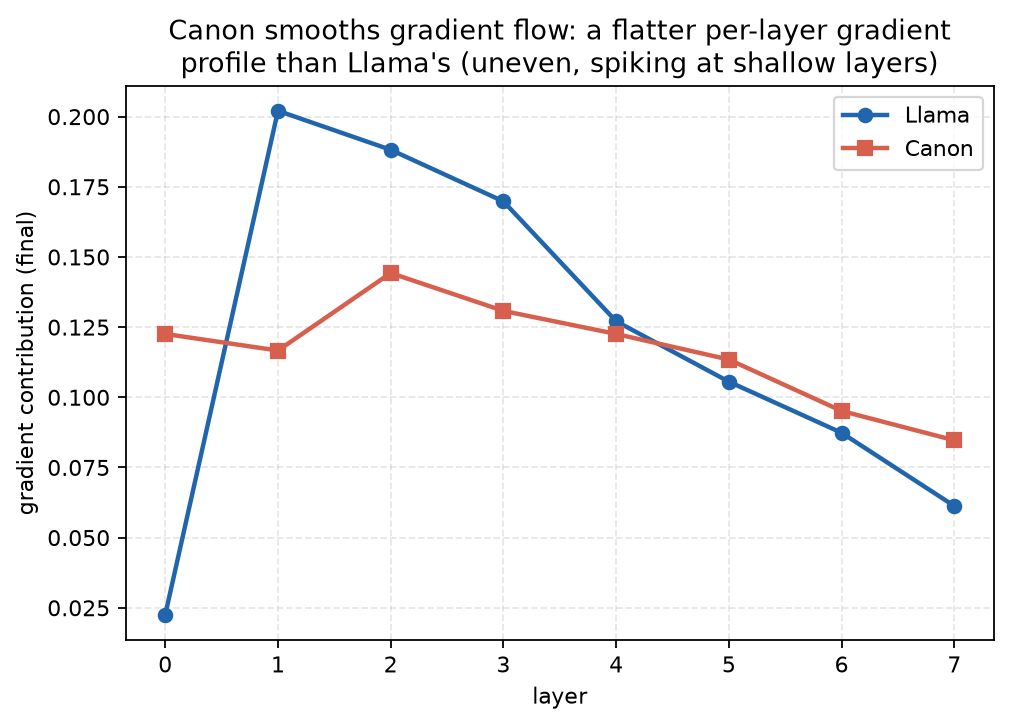
\includegraphics[width=\linewidth]{grad_profile.png}
      \begin{center}\small \textbf{Gradient smoothing:} per-layer gradient contribution\end{center}
    \column{0.5\textwidth}
      
\includegraphics[width=\linewidth]{rms_ratio.png}
      \begin{center}\small \textbf{Representation upscaling:} Canon conv output/input RMS ratio\end{center}
  \end{columns}
  \vspace{0.2em}
  \begin{itemize}
    \item \textbf{Gradient smoothing:} Llama spikes at shallow layers and decays;
          Canon leaves a flatter gradient across layers
    \item \textbf{Representation upscaling:} the Canon conv amplifies the residual
          stream (RMS ratio $>1$), most strongly in the deep layers near the LM head.
  \end{itemize}
\end{frame}

% ------------------------------------------------------------------
% Slide 16 --- Mechanism 3: long-range inductive bias
% ------------------------------------------------------------------
\begin{frame}{Mechanism 3: Long-Range Mixing}
  \begin{columns}[T]
    \column{0.34\textwidth}
      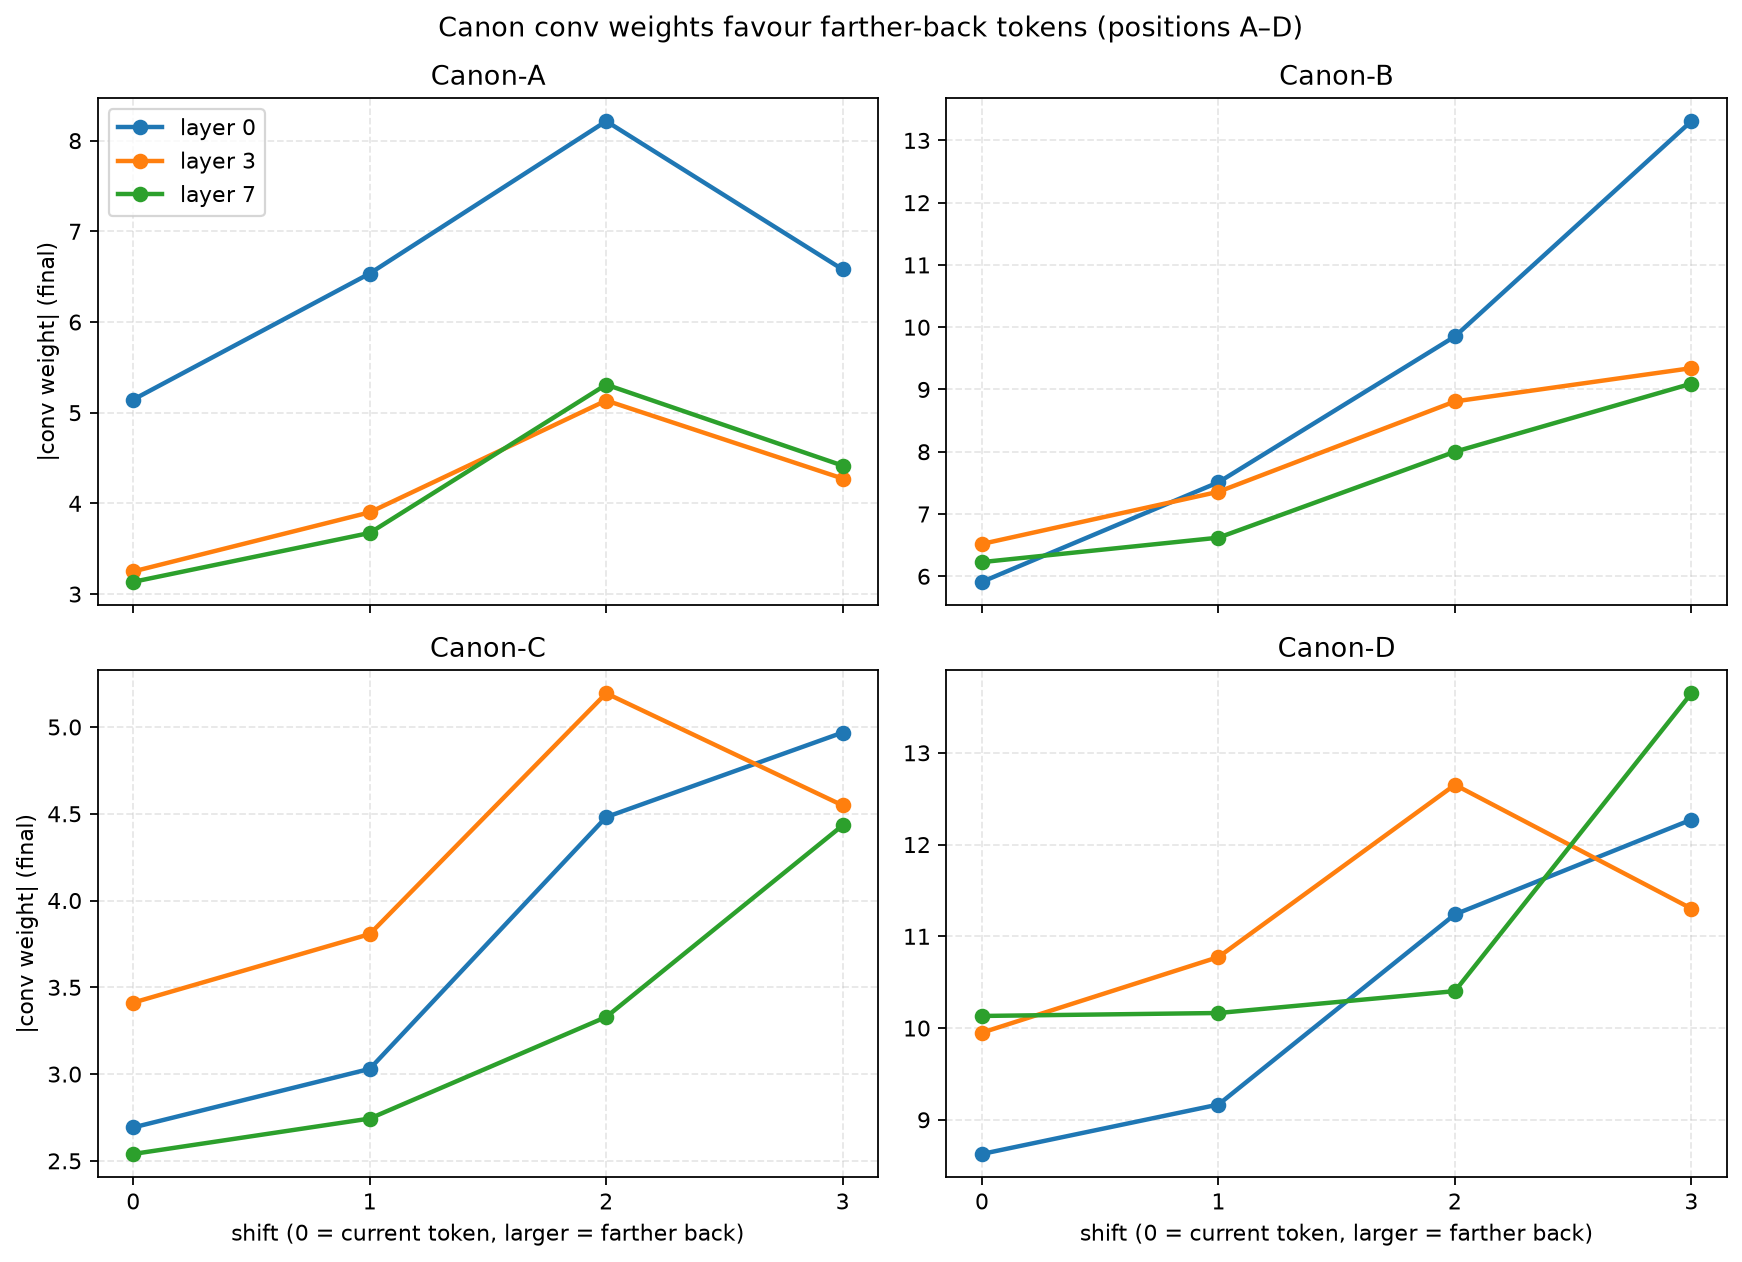
\includegraphics[width=\linewidth]{canon_weights.png}
    \column{0.33\textwidth}
      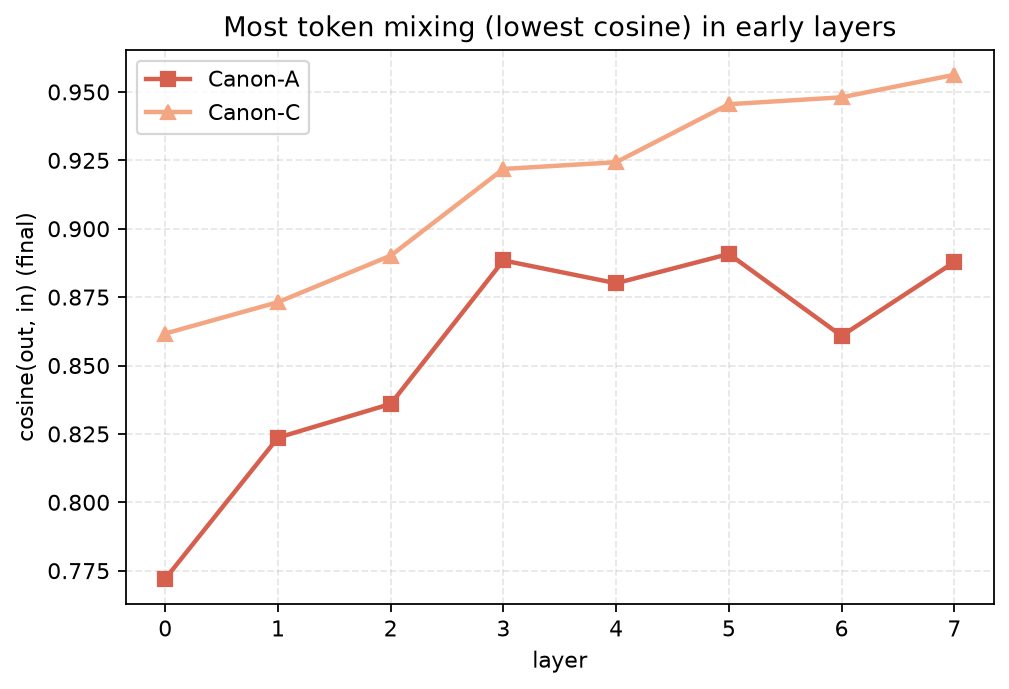
\includegraphics[width=\linewidth]{cos_sim.png}
    \column{0.33\textwidth}
      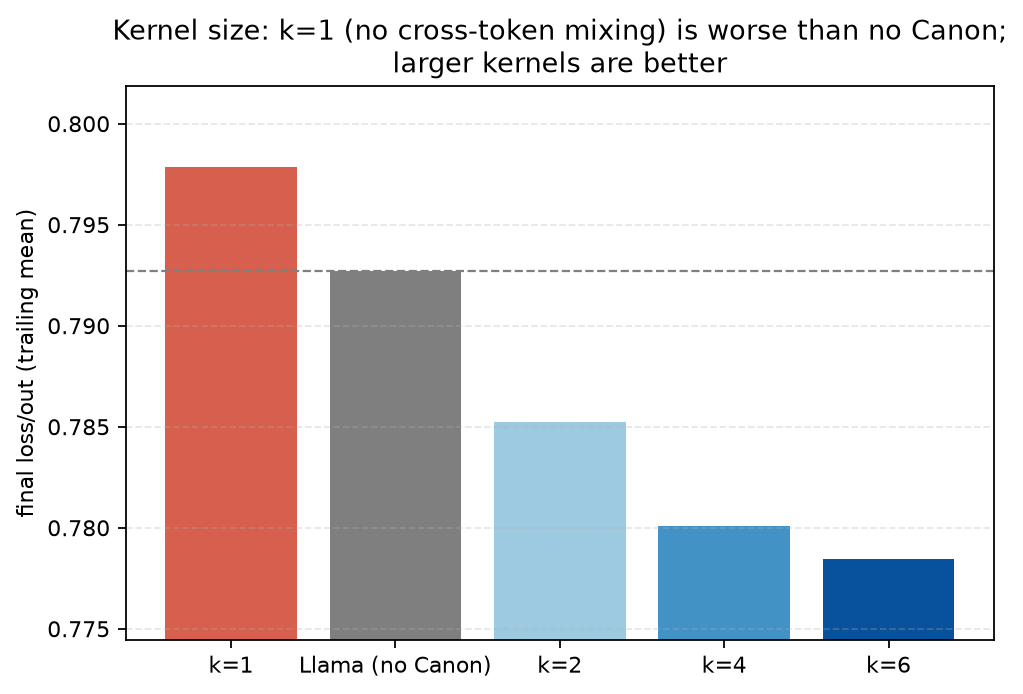
\includegraphics[width=\linewidth]{kernel.png}
  \end{columns}
  \vspace{0.2em}
  \begin{itemize}
    \item \textbf{Farther-back preference:} Further tokens contribute more
          tokens (shift $2>$ shift $0$)
    \item \textbf{Where it acts:} cross-token mixing is strongest in the early layers
          (lowest output/input cosine).
    \item \textbf{Necessity:} $k{=}1$ (no cross-token mixing) is worse than basline;
          loss improves monotonically as the kernel widens.
  \end{itemize}
\end{frame}

% ------------------------------------------------------------------
% Slide 17 --- Summary of the three mechanisms
% ------------------------------------------------------------------
\begin{frame}{Three Mechanistic Signatures: Summary}
  \vspace{0.6em}
  \begin{itemize}
    \item \textbf{Gradient redistribution.} Canon rescales the representations and smoothens the gradient across depth.
    \item \textbf{Long-range inductive bias.} Learned weights favour farther-back tokens
          from initialisation; mixing is strongest in early layers, and removing it
          ($k{=}1$) is worse than no Canon at all.
  \end{itemize}

  \vspace{0.6em}
  $\Rightarrow$ Additional horizontal information mixing is the primary contribution of Canon. \\
  $\Rightarrow$ Depth reasoning tasks benefit most from this.
\end{frame}


% ==================================================================
\section{Recommended Configuration}
% ==================================================================

% ------------------------------------------------------------------
% Ablation 1 --- Kernel size ablation
% ------------------------------------------------------------------
\begin{frame}{Ablation: Kernel Size}
  \begin{columns}[T]
    \column{0.55\textwidth}
      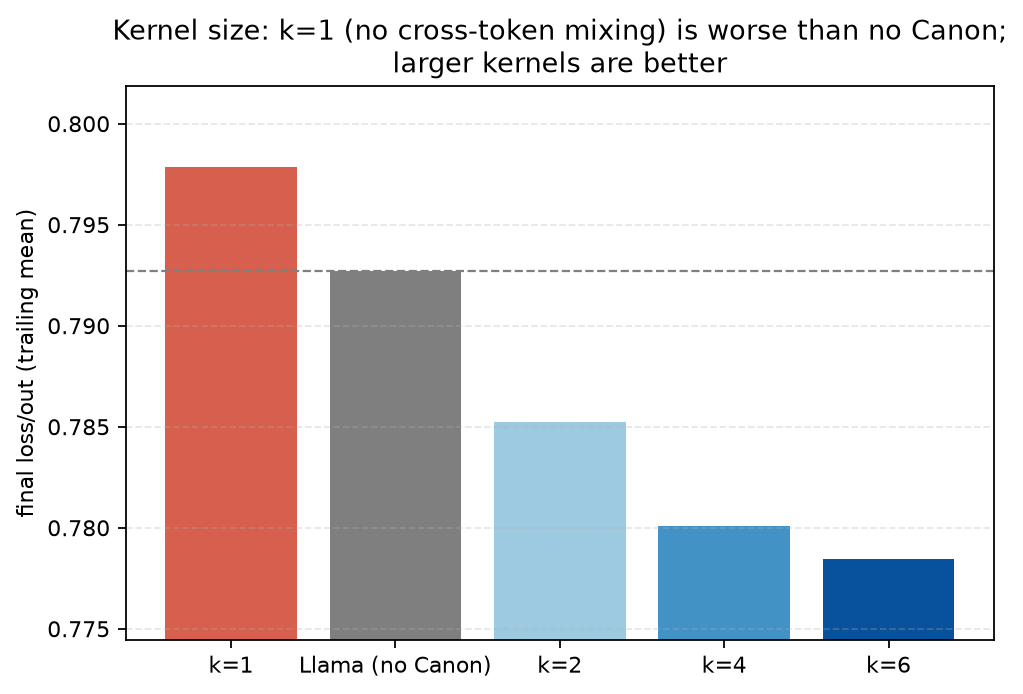
\includegraphics[width=\linewidth]{kernel.png}
    \column{0.43\textwidth}
      \textbf{Sweep $k \in \{1,2,4,6\}$} on text modelling (Llama baseline dashed).

      \vspace{0.5em}
      \begin{itemize}
        \item $k{=}1$ is worse than no Canon: a pointwise gate that hurts.
        \item Loss falls monotonically with $k$, saturating by $k{=}4$ to $6$.
        \item Cross-token mixing, not extra parameters, drives the gain.
      \end{itemize}
  \end{columns}
\end{frame}

% ------------------------------------------------------------------
% Ablation 2 --- Position ablation
% ------------------------------------------------------------------
\begin{frame}{Ablation: Insertion Position (Canon-AC vs.\ ABCD)}
  \begin{columns}[T]
    \column{0.55\textwidth}
      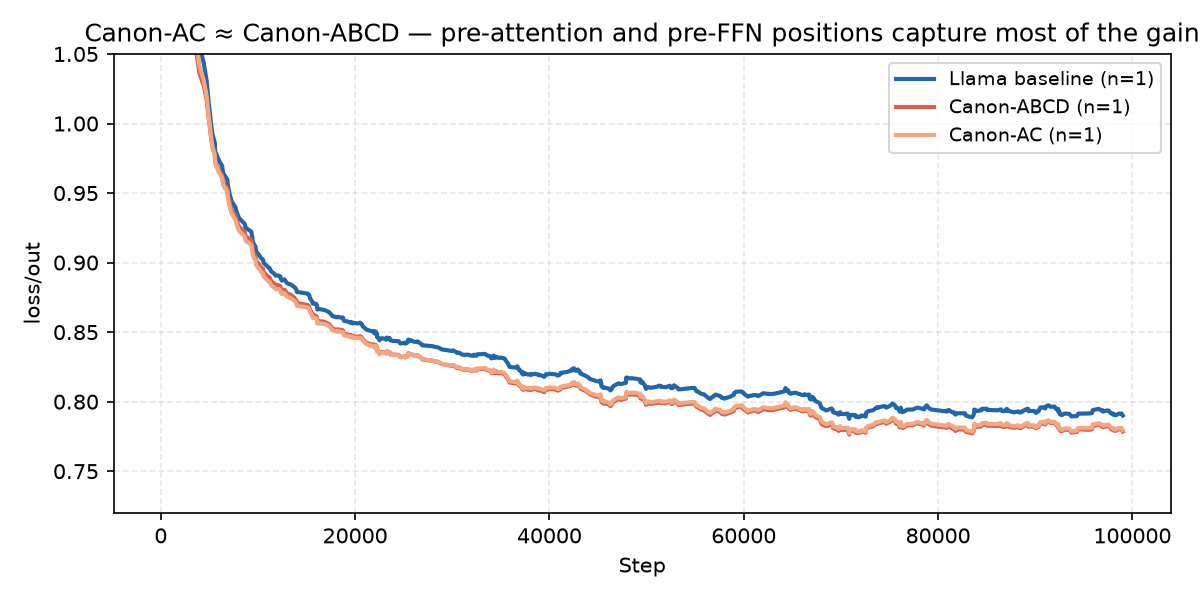
\includegraphics[width=\linewidth]{ac_vs_abcd.png}
    \column{0.43\textwidth}
      \textbf{Four insertion points per block} (A/B/C/D).

      \vspace{0.4em}
      Positions A (pre-attention) $+$ C (pre-FFN) recover essentially the full gain.

      \vspace{0.4em}
      \begin{center}
      \begin{tabular}{@{}lr@{}}
        \toprule
        Config & Loss \\
        \midrule
        Llama   & 0.793 \\
        Canon-AC & 0.782 \\
        Canon-ABCD & 0.781 \\
        \bottomrule
      \end{tabular}
      \end{center}
  \end{columns}
\end{frame}

% ------------------------------------------------------------------
% Ablation 3 --- Initialisation ablation
% ------------------------------------------------------------------
\begin{frame}{Ablation: Initialisation}
  \begin{columns}[T]
    \column{0.55\textwidth}
      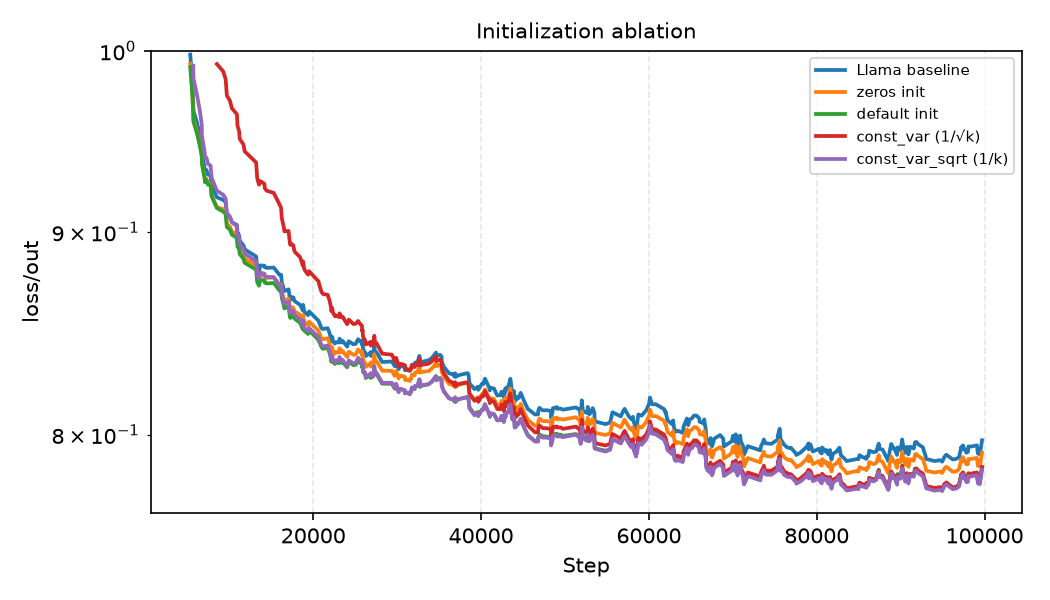
\includegraphics[width=\linewidth]{initialization.png}
    \column{0.43\textwidth}
      \textbf{All init schemes} (zeros, default, const\_var, $1/k$) outperform the
      Llama baseline.

      \vspace{0.5em}
      Initializing with mean is the best and better than default.

  \end{columns}
\end{frame}

% ------------------------------------------------------------------
% Slide --- Recommended Canon configuration (ablations summarised)
% ------------------------------------------------------------------
\begin{frame}{Recommended Configuration}
  Optimal configuration from ablations on text:

  \vspace{0.6em}
  \begin{itemize}
    \item \textbf{Kernel size $k \ge 4$.} Cross-token mixing is necessary:
          $k{=}1$ is worse than no Canon, and the gain saturates by $k\approx4$ to $6$.
    \item \textbf{Positions A + C} (pre-attention $+$ pre-FFN). These recover nearly the full
          gain of Canon-ABCD;
    \item \textbf{Initialisation: any scheme.} The benefit is init-agnostic
  \end{itemize}

  \vspace{0.6em}
  Recommended configuration: \textbf{Canon-AC, $k{=}4$, default init}.
\end{frame}


% ==================================================================
\section{Findings}
% ==================================================================

% ------------------------------------------------------------------
% Slide 17 --- Findings summary
% ------------------------------------------------------------------
\begin{frame}{Findings}
  \small
  \textbf{The benchmarks}
  \begin{itemize}
    \item Synthetic benchmarks are noisy: evaluating architectural changes requires multiple runs,
          no possibility to reason about the mechanism.
    \item Variance is tied with grokking
    \item ConComp is an alternative depth probe to Depo: similar capabilties, correlated with Depo,
          but far less noisy.
  \end{itemize}
  \vspace{0.2em}
  \textbf{Canon}
  \begin{itemize}
    \item Better at every scale (gap largest at small scale); gain
          concentrated on Depo and ConComp - depth reasoning tasks.
    \item \textbf{Optimal configuration:} Canon-AC, $k{=}4$, default init.
          A+C recover the full gain, can be initialized with mean or zero.
    \item The primary effect of Canon comes from information mixing, not just from scaling.
  \end{itemize}
\end{frame}


% ==================================================================
\section{Discussion}
% ==================================================================

% ------------------------------------------------------------------
% Slide 18 --- Open Questions / Future work
% ------------------------------------------------------------------
\begin{frame}{Open Questions \& Future Work}
  \begin{itemize}
    \item The effect of adding horizontal information mixing by increasing the number of layers within the model.
    \item Design of robust synthetic tasks for depth reasoning and their alignment with text modeling.
  \end{itemize}
\end{frame}

% ------------------------------------------------------------------
% Slide 19 --- Thank you
% ------------------------------------------------------------------
\begin{frame}
  \begin{center}
    {\Huge Thank you!}
  \end{center}
\end{frame}


\end{document}
